\title{Inferencing From Bayesian Networks\\Lab 5}
\author{
Aditya Gupta \\
\underline{2015CSB1003}
\and
Milan Chaudhary\\
\underline{2015CSB1010}
}
\date{\today}

\documentclass[12pt]{article}

\usepackage{tikz}
\usetikzlibrary{datavisualization}

\begin{document}
\maketitle

\section{Introduction}
In this Lab exercise, we implemented the inference from Bayesian Networks using
\begin{itemize}
    \item Variable Elimination: which is an exact inference. It takes much space and time.
    \item Rejection Sampling: which is an approximated inference. It's a highly efficient algorithm, that reduces required time and space for large number of variables.
\end{itemize}

\section{Variable Elimination}
In this section of program, first a container with all the conditional probability tables from each node instantiated by the evidence varaibles were collected. Then for each hidden variable, all the factors with that variable in it was collected and joined together. This process was repeated until all hidden variables were joined (and summed). The result was thus the required row (after normalization) of the factor formed from joining all the remaining factors.

\subsection{Reduce}
For each row the index (in binary) was masked with 1 for all non-evidence variables. This leaves behind only the evidence variables and all must thus have same transformed value since evidence are given. Thus comparison was done and required rows were collected.

\subsection{Join}
In this operation the resultant factor will have union of all variables in both the factors, further the order of the variables is important. First the common variables were collected then the remaining variables from first then second factor. Both the tables were sorted by creating weights (for common variables) and performing a stable sort (for the remaining variables). The sort involved sorting indices instead of the whole table and then for each set of values for common variables, taken as a block, and the remaining variables's value from both factors for each block were taken and the result were calculated for each block by two nested loops.

\subsection{Sum}
We note that for summing over a variable's particular value, the value of the variable in the factor only changes periodically; the period was found out and then a hopping loop summed the probabilities for each value, thus finally eliminating the variable.

\subsection{Normalize}
The sum of the probabilities should be one, thus each row in the resultant factor was divided by the sum of probabilities of the whole factor.

\section{Rejection Sampling}
In this section of program, it will first take the topologically sorted variable list. It will sample the variable one by one from left to right in the list, which means that parents will be sampled before the child variable.
This process will be done iteratively for a long finite time. In this process rejection will happen as soon as the evidences gets wrong value and will not be counted for probability calculations.
The conditional probability of query variables are calculated using the non-rejected number of iterations and number of occurrences of the different values of query variables, which will be stored as a table representing probabilities of all possible value pairs of query variables.
Then it will just pick the given value pair of query variables, which is the answer of input query.

Note: If the evidence value collection is not possible it will answer ``These evidences don't occur at the same time, i.e. P(e) = 0, thus \(P(Q|e)\) is undefined''
as
\[P(Q|e)=\frac{P(Q,e)}{P(e)}\]
where $P(Q,e)$ and $P(e)$ are $0$.

\subsection{Convergence of the probabilities as function of\\ number of samples generated}
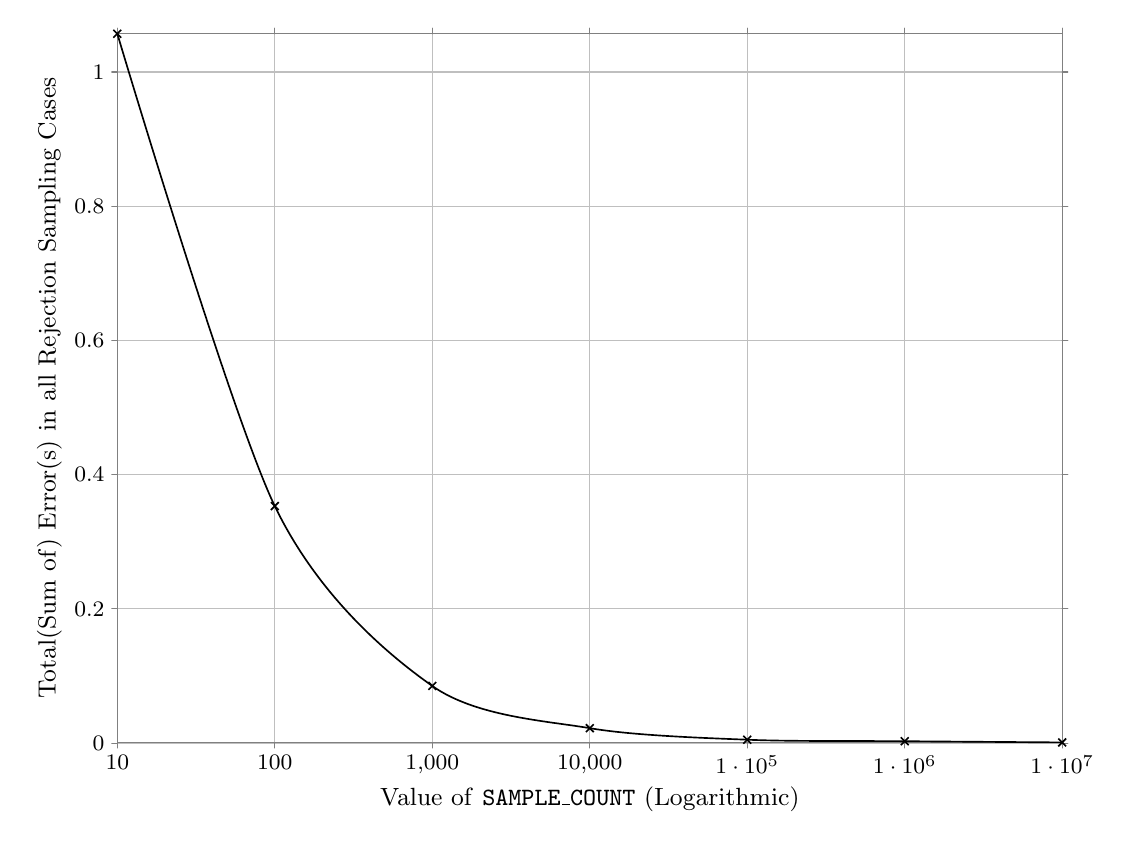
\begin{tikzpicture}
    \datavisualization [scientific axes,
    						 x axis={logarithmic,length=12cm,label=Value of \texttt{SAMPLE\_COUNT} (Logarithmic),grid},
     						 y axis={length=9cm,label=Total(Sum of) Error(s) in all Rejection Sampling Cases,grid},
    						 visualize as smooth line=my data,
    						 my data={style={mark=x}}]
    data {
        x, y
        10, 1.056972
        100, 0.353125
        1000, 0.085168
        10000, 0.022263
        100000, 0.005043
        1000000, 0.002833
        10000000,  0.0010175
    };
\end{tikzpicture}

\end{document}
